\documentclass[DM,toc,lsstdraft]{lsstdoc}
% lsstdoc documentation: https://lsst-texmf.lsst.io/lsstdoc.html
\usepackage{geometry}
\usepackage{longtable,booktabs,graphicx}
\usepackage{enumitem}
\usepackage{arydshln}

% Generated by Makefile
\input{meta}

% Package imports go here.

% Local commands go here.

% If you want glossaries, uncomment:
% \input{aglossary.tex}
% \makeglossaries

\title{Characterization Metric Report: Science Pipelines Version 27.0.0}
% \setDocSubtitle{Optional subtitle}

\author{%
Jeff Carlin
}

\setDocRef{DMTR-431}
\setDocUpstreamLocation{\url{https://github.com/lsst-dm/DMTR-431}}
\date{\vcsDate}
% \setDocCurator{The Curator of this Document}

\setDocAbstract{%
This brief report describes measurements of data quality metrics that were carried out for release v27.0.0 of the LSST Science Pipelines. The report for the previous version can be found in \citedsp{DMTR-421}.
}

% Revision history.
% Order: oldest first.
% Fields: VERSION, DATE, DESCRIPTION, OWNER NAME.
% See LPM-51 for version number policy.
\setDocChangeRecord{%
  \addtohist{1}{2024-06-05}{Unreleased.}{Jeff Carlin}
}

\begin{document}

\maketitle

% ADD CONTENT HERE
% You can also use the \input command to include several content files.
In this report, we characterize the performance of the Rubin Observatory Science Pipelines Version 27.0.0. We illustrate the performance via metrics that are measured on the HSC-RC2 dataset. RC2 consists of 3 tracts of data taken from the HSC-SSP survey, and selected to provide a means of testing various ``pathological'' cases (e.g., difficult astrometric solutions, extremely good seeing that does not provide a well-sampled PSF, difficult fields for deblending, and large galaxies, among others). These three tracts each contain between 112--149 visits split between the HSC-G, HSC-R, HSC-I, HSC-Z, and HSC-Y (\emph{grizy}) filters.

Between w\_2023\_32 (the source for pipelines version 26) and w\_2024\_16 (v27 source), most major changes have been in the pipelines ``middleware'' and other pipelines infrastructure, with few changes that would be expected to affect the results of data processing.
The major change that is expected to affect data products is the adoption of a modified form of \href{https://github.com/lsst/gbdes}{gbdes} for determining astrometric solutions in the pipelines. This was accompanied by a switch from using Gaia DR2 to DR3 as the astrometric reference catalog.
However, as shown in this document, the adoption of \texttt{gbdes} did not lead to significant changes in the astrometry metrics as measured on RC2.
As further adaptation and refinement of \texttt{gbdes} continues we expect to see improvements in these metrics.

All metrics reported here were calculated using the \href{https://github.com/lsst/faro}{faro} (\citeds{DMTN-211}) metric calculation package, which is part of the standard pipeline builds. All of the underlying algorithms to calculate metrics within \texttt{faro} are the same as they were in v25.0.0 of the Science Pipelines, so any differences between metrics from the v25 and v26 releases are due to changes in the underlying pipelines.

The metric calculation pipelines from \texttt{faro} were run on the RC2 tracts to derive the photometric, astrometric, and shape metrics that are reported here. We exclude the two astrometry metrics (AM3 and AF3) that concern residuals on 200-arcminute scales, since the individual tracts of RC2 do not span large enough spatial scales to enable these measurements.

For comparison, we provide the \SRD required ``design'' value of each Key Performance Metric (KPM) as defined in the Science Requirements Document \citedsp{LPM-17}. For the ellipticity correlation metrics, there are specifications only for \emph{r} and \emph{i} bands. The \emph{ugzy}-band measurements are of interest primarily for historical tracking.

Some KPMs (e.g., PF1, AF1, AF2) involve thresholds that are different for ``design'', ``minimum'', and ``stretch'' specifications. Metrics in this report are all compared to the ``design'' thresholds. The assessment of these KPMs would be different if evaluated against different thresholds.

\begin{figure}[!t]
  \centering
  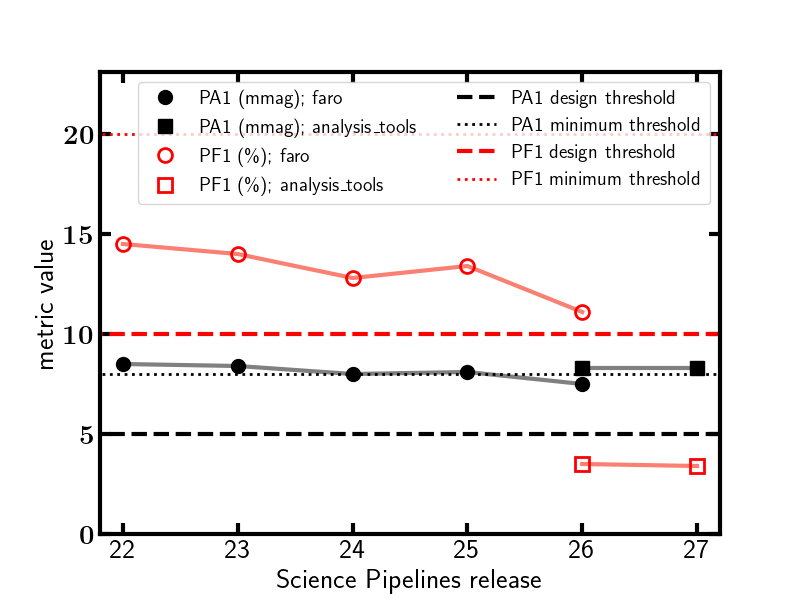
\includegraphics[width=0.6\textwidth, trim=0.0in 0.0in 0.0in 0.0in, clip]{figures/photom_metrics_v27_with_thresholds.png}
  \caption{Photometry metrics PA1 (photometric repeatability) and PF1 (percentage of measurements exceeding the outlier threshold) measured in the $r$-band. The figure shows the values of these metrics as measured with \texttt{faro} in versions 22-26 of the LSST Science Pipelines as circles, compared against the SRD requirements (for both the ``design'' and ``minimum'' thresholds). The measurements from \texttt{analysis\_tools} in versions 26-27 of the Science Pipelines are shown as squares. The measured values of both metrics are unchanged between the two most recent releases (v26 and v27). The algorithm to calculate PA1 is unchanged between \texttt{faro} and \texttt{analysis\_tools} (though because of differences in software architecture, it is expected that we would see minor differences in their outputs), and the metric differs by only a small offset between the two versions calculated in v26. However, while porting the PF1 metric to \texttt{analysis\_tools}, we discovered an error in the method of calculation (see the text for details). Fixing this error reduced the value of PF1 significantly.}
  \label{fig:phot_metrics}
\end{figure}

\section{Summary of performance metrics}

As noted previously, we now report metrics calculated by the \texttt{analysis\_tools} package, which improves upon the \texttt{faro} tools we had been previously using for calculation of data quality metrics. The plots in this Report include metrics from both \texttt{analysis\_tools} and \texttt{faro} for historical continuity, but future data processing campaigns will not run the \texttt{faro} tasks. One significant change is evident when comparing the outputs of the two frameworks on the v26 dataset: in Figure~\ref{fig:phot_metrics}, PF1 is much smaller as measured by \texttt{analysis\_tools} than from \texttt{faro}. This is expected, as we discovered an error in the calculation that was fixed when porting the PF1 metric from \texttt{faro} to \texttt{analysis\_tools} (see \href{https://rubinobs.atlassian.net/browse/DM-39332}{Jira ticket DM-39332} for details). The previous version had been calculating the outlier fraction relative to a fixed value of 15 mmag, while the metric is intended to be the fraction of outliers \textit{more than 15 mmag from the median} photometric repeatability. The changes on DM-39332 have brought the PF1 metric's calculation in line with the description in the DMSR, resulting in a value that is well beneath the design threshold for PF1.

As noted in the previous section, most of the major changes between versions 25 and 26 of the pipelines are related to improvements in efficiency and other ``under the hood'' modifications. Other than the astrometric solver, the data processing algorithms in the Science Pipelines are virtually unchanged between versions 25 and 26, so the data quality metrics should also be similar. In spite of the switch to a new astrometric code, the astrometry metrics (Section~\ref{astrometric-performance}) show only minor changes between the previous (v25) and current (v26) Science Pipelines releases.
The ellipticity correlation metrics (Section~\ref{ellipticity-correlations}) show only small differences between Release 25 and 26.

The photometry metrics (Section~\ref{photometric-performance}) improved significantly between v25 and v26, with the photometric repeatability (PA1) improving by 6-8\% in all bands, and the percentage of stars exceeding the outlier limit (PF1) improving by 15-20\% in all bands.
We believe the improvement came about from the bug fixes on \href{https://jira.lsstcorp.org/browse/DM-37955}{Jira ticket DM-37955}. This ticket addressed the fact that the fitting of aperture correction maps was not robust, and so outliers (due to blends, unmasked cosmic rays, etc.) would bias the map and thus increase the scatter in the aperture corrections, on a per-image basis. By using a fitting algorithm that was more robust to outliers we have reduced the scatter between the calibration flux (measured in 12-pixel apertures) and the PSF flux, and thus decreased the scatter in the photometric repeatability measured using PSF fluxes.
% All photometric calibration is run with “calibration flux” (currently aper12, will be compensated gaussian flux in the next few months).  To put the psf flux on the same scale as the calibration flux we measure an aperture correction map, which is a 2D second order Chebyshev polynomial mapping from one to the other.  This “aperture correction” is not to infinity, but rather to match the flux that has been well calibrated internally and versus external calibrators.
% DM-37955 addresses the fact that the aperture correction map fitting routine was not robust, and so outliers (due to blends, unmasked CRs, etc) would bias the map and thus increase the scatter between the calibration flux and the psf flux, on a per-image basis.  There are figures on the ticket if you need any.  By using a fitting algorithm that was more robust to outliers we could reduce the scatter between these two fluxes, and thus decrease the scatter in the photometric repeatability when using PSF fluxes.  This ticket should have no impact on the repeatability of the calibration flux.  At the same time, we want to use PSF fluxes for this metric because they have less noise and less residual background bias than large aperture fluxes.

\section{Photometric Performance}\label{photometric-performance}
% NOTE: In v28, add the calib flux repeatability!

These photometric performance metrics are defined in LSS-REQ-0093 (\citeds{LSE-29}) and Table 14 of \citeds{LPM-17}. Values in this table represent the mean of the results reported by \texttt{analysis\_tools} for the three tracts in RC2.

Any entries left blank are those for which we do not have data in the given filter for that dataset.

\begin{longtable}[]{@{}llllll@{}}
\toprule
\begin{minipage}[b]{0.12\columnwidth}\raggedright\strut
Metric\strut
\end{minipage} & \begin{minipage}[b]{0.06\columnwidth}\raggedright\strut
Unit\strut
\end{minipage} & \begin{minipage}[b]{0.14\columnwidth}\raggedright\strut
SRD Requirement -- Design\strut
\end{minipage} & \begin{minipage}[b]{0.12\columnwidth}\raggedright\strut
Release 26 Value (RC2) \strut
\end{minipage} & \begin{minipage}[b]{0.12\columnwidth}\raggedright\strut
Release 27 Value (RC2) \strut
\end{minipage} & \begin{minipage}[b]{0.17\columnwidth}\raggedright\strut
Comments\strut
\end{minipage}\tabularnewline
\midrule
\endhead
\begin{minipage}[t]{0.12\columnwidth}\raggedright\strut
PA1: \emph{u}\strut
\end{minipage} & \begin{minipage}[t]{0.06\columnwidth}\raggedright\strut
mmag\strut
\end{minipage} & \begin{minipage}[t]{0.14\columnwidth}\raggedright\strut
\(\leq 7.5\)\strut
\end{minipage} & \begin{minipage}[t]{0.12\columnwidth}\raggedright\strut
--- \strut
\end{minipage} & \begin{minipage}[t]{0.12\columnwidth}\raggedright\strut
--- \strut
\end{minipage} & \begin{minipage}[t]{0.17\columnwidth}\raggedright\strut
No data\strut
\end{minipage}\tabularnewline
\begin{minipage}[t]{0.12\columnwidth}\raggedright\strut
PA1: \emph{g}\strut
\end{minipage} & \begin{minipage}[t]{0.06\columnwidth}\raggedright\strut
mmag\strut
\end{minipage} & \begin{minipage}[t]{0.14\columnwidth}\raggedright\strut
\(\leq 5.0\)\strut
\end{minipage} & \begin{minipage}[t]{0.12\columnwidth}\raggedright\strut
7.2 \strut
\end{minipage} & \begin{minipage}[t]{0.12\columnwidth}\raggedright\strut
7.9 \strut
\end{minipage} & \begin{minipage}[t]{0.17\columnwidth}\raggedright\strut
\strut
\end{minipage}\tabularnewline
\begin{minipage}[t]{0.12\columnwidth}\raggedright\strut
PA1: \emph{r}\strut
\end{minipage} & \begin{minipage}[t]{0.06\columnwidth}\raggedright\strut
mmag\strut
\end{minipage} & \begin{minipage}[t]{0.14\columnwidth}\raggedright\strut
\(\leq 5.0\)\strut
\end{minipage} & \begin{minipage}[t]{0.12\columnwidth}\raggedright\strut
8.3\strut
\end{minipage} & \begin{minipage}[t]{0.12\columnwidth}\raggedright\strut
8.3\strut
\end{minipage} & \begin{minipage}[t]{0.17\columnwidth}\raggedright\strut
\strut
\end{minipage}\tabularnewline
\begin{minipage}[t]{0.12\columnwidth}\raggedright\strut
PA1: \emph{i}\strut
\end{minipage} & \begin{minipage}[t]{0.06\columnwidth}\raggedright\strut
mmag\strut
\end{minipage} & \begin{minipage}[t]{0.14\columnwidth}\raggedright\strut
\(\leq 5.0\)\strut
\end{minipage} & \begin{minipage}[t]{0.12\columnwidth}\raggedright\strut
8.6\strut
\end{minipage} & \begin{minipage}[t]{0.12\columnwidth}\raggedright\strut
8.7\strut
\end{minipage} & \begin{minipage}[t]{0.17\columnwidth}\raggedright\strut
\strut
\end{minipage}\tabularnewline
\begin{minipage}[t]{0.12\columnwidth}\raggedright\strut
PA1: \emph{z}\strut
\end{minipage} & \begin{minipage}[t]{0.06\columnwidth}\raggedright\strut
mmag\strut
\end{minipage} & \begin{minipage}[t]{0.14\columnwidth}\raggedright\strut
\(\leq 7.5\)\strut
\end{minipage} & \begin{minipage}[t]{0.12\columnwidth}\raggedright\strut
6.7\strut
\end{minipage} & \begin{minipage}[t]{0.12\columnwidth}\raggedright\strut
6.7\strut
\end{minipage} & \begin{minipage}[t]{0.17\columnwidth}\raggedright\strut
\strut
\end{minipage}\tabularnewline
\begin{minipage}[t]{0.12\columnwidth}\raggedright\strut
PA1: \emph{y}\strut
\end{minipage} & \begin{minipage}[t]{0.06\columnwidth}\raggedright\strut
mmag\strut
\end{minipage} & \begin{minipage}[t]{0.14\columnwidth}\raggedright\strut
\(\leq 7.5\)\strut
\end{minipage} & \begin{minipage}[t]{0.12\columnwidth}\raggedright\strut
7.3\strut
\end{minipage} & \begin{minipage}[t]{0.12\columnwidth}\raggedright\strut
7.3\strut
\end{minipage} & \begin{minipage}[t]{0.17\columnwidth}\raggedright\strut
\strut
\end{minipage}\tabularnewline
\begin{minipage}[t]{0.12\columnwidth}\raggedright\strut
PF1: \emph{u}\strut
\end{minipage} & \begin{minipage}[t]{0.06\columnwidth}\raggedright\strut
\%\strut
\end{minipage} & \begin{minipage}[t]{0.14\columnwidth}\raggedright\strut
\(\leq 20\)\strut
\end{minipage} & \begin{minipage}[t]{0.12\columnwidth}\raggedright\strut
---\strut
\end{minipage} & \begin{minipage}[t]{0.12\columnwidth}\raggedright\strut
---\strut
\end{minipage} & \begin{minipage}[t]{0.17\columnwidth}\raggedright\strut
No data\strut
\end{minipage}\tabularnewline
\begin{minipage}[t]{0.12\columnwidth}\raggedright\strut
PF1: \emph{g}\strut
\end{minipage} & \begin{minipage}[t]{0.06\columnwidth}\raggedright\strut
\%\strut
\end{minipage} & \begin{minipage}[t]{0.14\columnwidth}\raggedright\strut
\(\leq 20\)\strut
\end{minipage} & \begin{minipage}[t]{0.12\columnwidth}\raggedright\strut
6.3\strut
\end{minipage} & \begin{minipage}[t]{0.12\columnwidth}\raggedright\strut
4.4\strut
\end{minipage} & \begin{minipage}[t]{0.17\columnwidth}\raggedright\strut
\strut
\end{minipage}\tabularnewline
\begin{minipage}[t]{0.12\columnwidth}\raggedright\strut
PF1: \emph{r}\strut
\end{minipage} & \begin{minipage}[t]{0.06\columnwidth}\raggedright\strut
\%\strut
\end{minipage} & \begin{minipage}[t]{0.14\columnwidth}\raggedright\strut
\(\leq 10\)\strut
\end{minipage} & \begin{minipage}[t]{0.12\columnwidth}\raggedright\strut
3.5\strut
\end{minipage} & \begin{minipage}[t]{0.12\columnwidth}\raggedright\strut
3.4\strut
\end{minipage} & \begin{minipage}[t]{0.17\columnwidth}\raggedright\strut
\strut
\end{minipage}\tabularnewline
\begin{minipage}[t]{0.12\columnwidth}\raggedright\strut
PF1: \emph{i}\strut
\end{minipage} & \begin{minipage}[t]{0.06\columnwidth}\raggedright\strut
\%\strut
\end{minipage} & \begin{minipage}[t]{0.14\columnwidth}\raggedright\strut
\(\leq 10\)\strut
\end{minipage} & \begin{minipage}[t]{0.12\columnwidth}\raggedright\strut
2.5\strut
\end{minipage} & \begin{minipage}[t]{0.12\columnwidth}\raggedright\strut
2.8\strut
\end{minipage} & \begin{minipage}[t]{0.17\columnwidth}\raggedright\strut
\strut
\end{minipage}\tabularnewline
\begin{minipage}[t]{0.12\columnwidth}\raggedright\strut
PF1: \emph{z}\strut
\end{minipage} & \begin{minipage}[t]{0.06\columnwidth}\raggedright\strut
\%\strut
\end{minipage} & \begin{minipage}[t]{0.14\columnwidth}\raggedright\strut
\(\leq 20\)\strut
\end{minipage} & \begin{minipage}[t]{0.12\columnwidth}\raggedright\strut
1.5\strut
\end{minipage} & \begin{minipage}[t]{0.12\columnwidth}\raggedright\strut
1.6\strut
\end{minipage} & \begin{minipage}[t]{0.17\columnwidth}\raggedright\strut
\strut
\end{minipage}\tabularnewline
\begin{minipage}[t]{0.12\columnwidth}\raggedright\strut
PF1: \emph{y}\strut
\end{minipage} & \begin{minipage}[t]{0.06\columnwidth}\raggedright\strut
\%\strut
\end{minipage} & \begin{minipage}[t]{0.14\columnwidth}\raggedright\strut
\(\leq 10\)\strut
\end{minipage} & \begin{minipage}[t]{0.12\columnwidth}\raggedright\strut
1.8\strut
\end{minipage} & \begin{minipage}[t]{0.12\columnwidth}\raggedright\strut
2.2\strut
\end{minipage} & \begin{minipage}[t]{0.17\columnwidth}\raggedright\strut
\strut
\end{minipage}\tabularnewline
\bottomrule
\end{longtable}

\section{Astrometric Performance}\label{astrometric-performance}

\begin{figure}[!t]
  \centering
  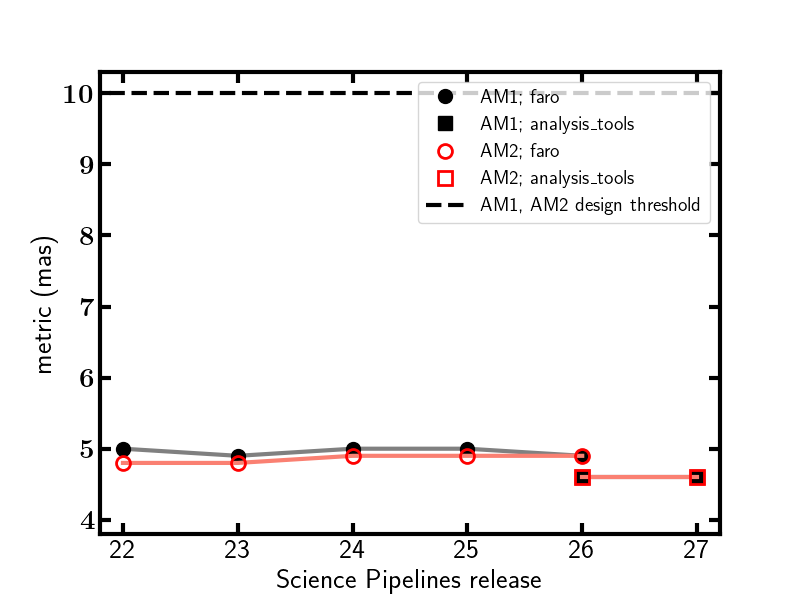
\includegraphics[width=0.475\textwidth, trim=0.0in 0.0in 0.0in 0.0in, clip]{figures/astrom_metrics_v27_with_thresholds.png}
  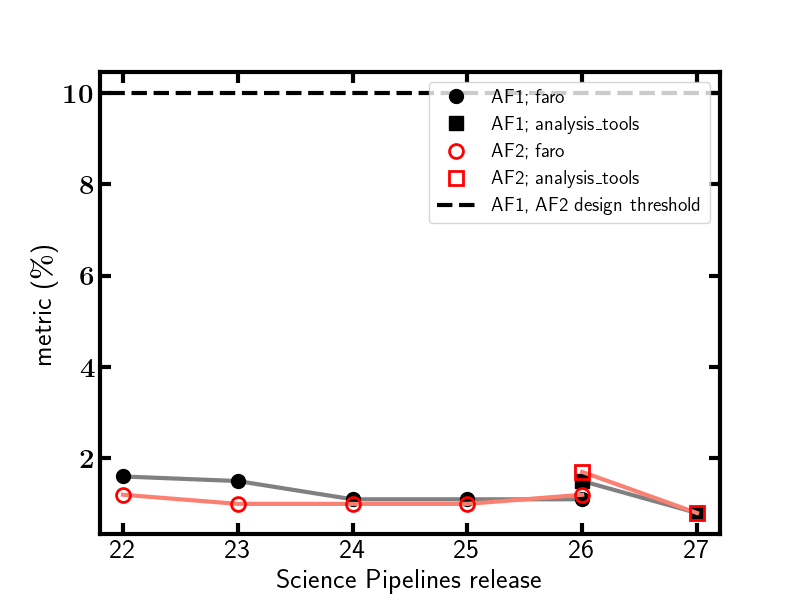
\includegraphics[width=0.475\textwidth, trim=0.0in 0.0in 0.0in 0.0in, clip]{figures/astrom_outlier_metrics_v27_with_thresholds.png}
  \caption{Astrometry metrics measured on $r$-band images compared over the past few major pipelines releases. \textit{Left: } Median astrometric measurement error on 5-arcminute scales (AM1) and 20-arcminute scales (AM2), compared against the SRD requirements (for the ``design'' thresholds; note that the thresholds for AM1 and AM2 are the same, and thus indistinguishable on the figure). \textit{Right: } Fraction of astrometric measurements exceeding the outlier threshold on 5-arcminute (AF1) and 20-arcminute (AF2) scales, compared against the SRD requirements (for the ``design'' thresholds; note that the thresholds for AF1 and AF2 are the same, and thus indistinguishable on the figure). The measured values of these metrics were virtually unchanged between pipelines version 25 and v26, which is surprising given the adoption of a new astrometric solver in the pipelines. We expect that further refinements of the \texttt{gbdes} astrometry algorithms will improve the astrometry metrics in the future. }
  \label{fig:astrom_metrics}
\end{figure}

The following metrics are defined following LSR-REQ-0094
\citedsp{LSE-29} and Table 18 of \citeds{LPM-17}. Values in this table represent the mean of the results reported by \texttt{faro} for the three tracts in RC2.

Any entries left blank are those for which we do not have data in the given filter for that dataset.

\begin{longtable}[]{@{}llllll@{}}
\toprule
\begin{minipage}[b]{0.12\columnwidth}\raggedright\strut
Metric\strut
\end{minipage} & \begin{minipage}[b]{0.06\columnwidth}\raggedright\strut
Unit\strut
\end{minipage} & \begin{minipage}[b]{0.14\columnwidth}\raggedright\strut
SRD Requirement -- Design\strut
\end{minipage} & \begin{minipage}[b]{0.12\columnwidth}\raggedright\strut
Release 26 Value (RC2)\strut
\end{minipage} & \begin{minipage}[b]{0.12\columnwidth}\raggedright\strut
Release 27 Value (RC2) \strut
\end{minipage} & \begin{minipage}[b]{0.17\columnwidth}\raggedright\strut
Comments\strut
\end{minipage}\tabularnewline
\midrule
\endhead
\begin{minipage}[t]{0.12\columnwidth}\raggedright\strut
AM1: \emph{u}\strut
\end{minipage} & \begin{minipage}[t]{0.06\columnwidth}\raggedright\strut
mas\strut
\end{minipage} & \begin{minipage}[t]{0.14\columnwidth}\raggedright\strut
\(\leq 10\)\strut
\end{minipage} & \begin{minipage}[t]{0.12\columnwidth}\raggedright\strut
---\strut
\end{minipage} & \begin{minipage}[t]{0.12\columnwidth}\raggedright\strut
--- \strut
\end{minipage} & \begin{minipage}[t]{0.17\columnwidth}\raggedright\strut
No data\strut
\end{minipage}\tabularnewline
\begin{minipage}[t]{0.12\columnwidth}\raggedright\strut
AM1: \emph{g}\strut
\end{minipage} & \begin{minipage}[t]{0.06\columnwidth}\raggedright\strut
mas\strut
\end{minipage} & \begin{minipage}[t]{0.14\columnwidth}\raggedright\strut
\(\leq 10\)\strut
\end{minipage} & \begin{minipage}[t]{0.12\columnwidth}\raggedright\strut
5.2\strut
\end{minipage} & \begin{minipage}[t]{0.12\columnwidth}\raggedright\strut
5.2 \strut
\end{minipage} & \begin{minipage}[t]{0.17\columnwidth}\raggedright\strut
\strut
\end{minipage}\tabularnewline
\begin{minipage}[t]{0.12\columnwidth}\raggedright\strut
AM1: \emph{r}\strut
\end{minipage} & \begin{minipage}[t]{0.06\columnwidth}\raggedright\strut
mas\strut
\end{minipage} & \begin{minipage}[t]{0.14\columnwidth}\raggedright\strut
\(\leq 10\)\strut
\end{minipage} & \begin{minipage}[t]{0.12\columnwidth}\raggedright\strut
4.6\strut
\end{minipage} & \begin{minipage}[t]{0.12\columnwidth}\raggedright\strut
4.6\strut
\end{minipage} & \begin{minipage}[t]{0.17\columnwidth}\raggedright\strut
\strut
\end{minipage}\tabularnewline
\begin{minipage}[t]{0.12\columnwidth}\raggedright\strut
AM1: \emph{i}\strut
\end{minipage} & \begin{minipage}[t]{0.06\columnwidth}\raggedright\strut
mas\strut
\end{minipage} & \begin{minipage}[t]{0.14\columnwidth}\raggedright\strut
\(\leq 10\)\strut
\end{minipage} & \begin{minipage}[t]{0.12\columnwidth}\raggedright\strut
4.0\strut
\end{minipage} & \begin{minipage}[t]{0.12\columnwidth}\raggedright\strut
4.1\strut
\end{minipage} & \begin{minipage}[t]{0.17\columnwidth}\raggedright\strut
\strut
\end{minipage}\tabularnewline
\begin{minipage}[t]{0.12\columnwidth}\raggedright\strut
AM1: \emph{z}\strut
\end{minipage} & \begin{minipage}[t]{0.06\columnwidth}\raggedright\strut
mas\strut
\end{minipage} & \begin{minipage}[t]{0.14\columnwidth}\raggedright\strut
\(\leq 10\)\strut
\end{minipage} & \begin{minipage}[t]{0.12\columnwidth}\raggedright\strut
5.2\strut
\end{minipage} & \begin{minipage}[t]{0.12\columnwidth}\raggedright\strut
5.2\strut
\end{minipage} & \begin{minipage}[t]{0.17\columnwidth}\raggedright\strut
\strut
\end{minipage}\tabularnewline
\begin{minipage}[t]{0.12\columnwidth}\raggedright\strut
AM1: \emph{y}\strut
\end{minipage} & \begin{minipage}[t]{0.06\columnwidth}\raggedright\strut
mas\strut
\end{minipage} & \begin{minipage}[t]{0.14\columnwidth}\raggedright\strut
\(\leq 10\)\strut
\end{minipage} & \begin{minipage}[t]{0.12\columnwidth}\raggedright\strut
6.9\strut
\end{minipage} & \begin{minipage}[t]{0.12\columnwidth}\raggedright\strut
6.9\strut
\end{minipage} & \begin{minipage}[t]{0.17\columnwidth}\raggedright\strut
\strut
\end{minipage}\tabularnewline
\begin{minipage}[t]{0.12\columnwidth}\raggedright\strut
AF1: \emph{u}\strut
\end{minipage} & \begin{minipage}[t]{0.06\columnwidth}\raggedright\strut
\%\strut
\end{minipage} & \begin{minipage}[t]{0.14\columnwidth}\raggedright\strut
\(\leq 10\)\strut
\end{minipage} & \begin{minipage}[t]{0.12\columnwidth}\raggedright\strut
---\strut
\end{minipage} & \begin{minipage}[t]{0.12\columnwidth}\raggedright\strut
---\strut
\end{minipage} & \begin{minipage}[t]{0.17\columnwidth}\raggedright\strut
No data\strut
\end{minipage}\tabularnewline
\begin{minipage}[t]{0.12\columnwidth}\raggedright\strut
AF1: \emph{g}\strut
\end{minipage} & \begin{minipage}[t]{0.06\columnwidth}\raggedright\strut
\%\strut
\end{minipage} & \begin{minipage}[t]{0.14\columnwidth}\raggedright\strut
\(\leq 10\)\strut
\end{minipage} & \begin{minipage}[t]{0.12\columnwidth}\raggedright\strut
1.6\strut
\end{minipage} & \begin{minipage}[t]{0.12\columnwidth}\raggedright\strut
0.9\strut
\end{minipage} & \begin{minipage}[t]{0.17\columnwidth}\raggedright\strut
\strut
\end{minipage}\tabularnewline
\begin{minipage}[t]{0.12\columnwidth}\raggedright\strut
AF1: \emph{r}\strut
\end{minipage} & \begin{minipage}[t]{0.06\columnwidth}\raggedright\strut
\%\strut
\end{minipage} & \begin{minipage}[t]{0.14\columnwidth}\raggedright\strut
\(\leq 10\)\strut
\end{minipage} & \begin{minipage}[t]{0.12\columnwidth}\raggedright\strut
1.5\strut
\end{minipage} & \begin{minipage}[t]{0.12\columnwidth}\raggedright\strut
0.8\strut
\end{minipage} & \begin{minipage}[t]{0.17\columnwidth}\raggedright\strut
\strut
\end{minipage}\tabularnewline
\begin{minipage}[t]{0.12\columnwidth}\raggedright\strut
AF1: \emph{i}\strut
\end{minipage} & \begin{minipage}[t]{0.06\columnwidth}\raggedright\strut
\%\strut
\end{minipage} & \begin{minipage}[t]{0.14\columnwidth}\raggedright\strut
\(\leq 10\)\strut
\end{minipage} & \begin{minipage}[t]{0.12\columnwidth}\raggedright\strut
0.9\strut
\end{minipage} & \begin{minipage}[t]{0.12\columnwidth}\raggedright\strut
0.6\strut
\end{minipage} & \begin{minipage}[t]{0.17\columnwidth}\raggedright\strut
\strut
\end{minipage}\tabularnewline
\begin{minipage}[t]{0.12\columnwidth}\raggedright\strut
AF1: \emph{z}\strut
\end{minipage} & \begin{minipage}[t]{0.06\columnwidth}\raggedright\strut
\%\strut
\end{minipage} & \begin{minipage}[t]{0.14\columnwidth}\raggedright\strut
\(\leq 10\)\strut
\end{minipage} & \begin{minipage}[t]{0.12\columnwidth}\raggedright\strut
1.2\strut
\end{minipage} & \begin{minipage}[t]{0.12\columnwidth}\raggedright\strut
0.6\strut
\end{minipage} & \begin{minipage}[t]{0.17\columnwidth}\raggedright\strut
\strut
\end{minipage}\tabularnewline
\begin{minipage}[t]{0.12\columnwidth}\raggedright\strut
AF1: \emph{y}\strut
\end{minipage} & \begin{minipage}[t]{0.06\columnwidth}\raggedright\strut
\%\strut
\end{minipage} & \begin{minipage}[t]{0.14\columnwidth}\raggedright\strut
\(\leq 10\)\strut
\end{minipage} & \begin{minipage}[t]{0.12\columnwidth}\raggedright\strut
3.8\strut
\end{minipage} & \begin{minipage}[t]{0.12\columnwidth}\raggedright\strut
2.9\strut
\end{minipage} & \begin{minipage}[t]{0.17\columnwidth}\raggedright\strut
\strut
\end{minipage}\tabularnewline
\begin{minipage}[t]{0.12\columnwidth}\raggedright\strut
AD1: \emph{u}\strut
\end{minipage} & \begin{minipage}[t]{0.06\columnwidth}\raggedright\strut
mas\strut
\end{minipage} & \begin{minipage}[t]{0.14\columnwidth}\raggedright\strut
\(\leq 20\)\strut
\end{minipage} & \begin{minipage}[t]{0.12\columnwidth}\raggedright\strut
---\strut
\end{minipage} & \begin{minipage}[t]{0.12\columnwidth}\raggedright\strut
---\strut
\end{minipage} & \begin{minipage}[t]{0.17\columnwidth}\raggedright\strut
No data\strut
\end{minipage}\tabularnewline
\begin{minipage}[t]{0.12\columnwidth}\raggedright\strut
AD1: \emph{g}\strut
\end{minipage} & \begin{minipage}[t]{0.06\columnwidth}\raggedright\strut
mas\strut
\end{minipage} & \begin{minipage}[t]{0.14\columnwidth}\raggedright\strut
\(\leq 20\)\strut
\end{minipage} & \begin{minipage}[t]{0.12\columnwidth}\raggedright\strut
10.5\strut
\end{minipage} & \begin{minipage}[t]{0.12\columnwidth}\raggedright\strut
9.7\strut
\end{minipage} & \begin{minipage}[t]{0.17\columnwidth}\raggedright\strut
\strut
\end{minipage}\tabularnewline
\begin{minipage}[t]{0.12\columnwidth}\raggedright\strut
AD1: \emph{r}\strut
\end{minipage} & \begin{minipage}[t]{0.06\columnwidth}\raggedright\strut
mas\strut
\end{minipage} & \begin{minipage}[t]{0.14\columnwidth}\raggedright\strut
\(\leq 20\)\strut
\end{minipage} & \begin{minipage}[t]{0.12\columnwidth}\raggedright\strut
9.7\strut
\end{minipage} & \begin{minipage}[t]{0.12\columnwidth}\raggedright\strut
9.2\strut
\end{minipage} & \begin{minipage}[t]{0.17\columnwidth}\raggedright\strut
\strut
\end{minipage}\tabularnewline
\begin{minipage}[t]{0.12\columnwidth}\raggedright\strut
AD1: \emph{i}\strut
\end{minipage} & \begin{minipage}[t]{0.06\columnwidth}\raggedright\strut
mas\strut
\end{minipage} & \begin{minipage}[t]{0.14\columnwidth}\raggedright\strut
\(\leq 20\)\strut
\end{minipage} & \begin{minipage}[t]{0.12\columnwidth}\raggedright\strut
8.1\strut
\end{minipage} & \begin{minipage}[t]{0.12\columnwidth}\raggedright\strut
7.9\strut
\end{minipage} & \begin{minipage}[t]{0.17\columnwidth}\raggedright\strut
\strut
\end{minipage}\tabularnewline
\begin{minipage}[t]{0.12\columnwidth}\raggedright\strut
AD1: \emph{z}\strut
\end{minipage} & \begin{minipage}[t]{0.06\columnwidth}\raggedright\strut
mas\strut
\end{minipage} & \begin{minipage}[t]{0.14\columnwidth}\raggedright\strut
\(\leq 20\)\strut
\end{minipage} & \begin{minipage}[t]{0.12\columnwidth}\raggedright\strut
10.2\strut
\end{minipage} & \begin{minipage}[t]{0.12\columnwidth}\raggedright\strut
9.7\strut
\end{minipage} & \begin{minipage}[t]{0.17\columnwidth}\raggedright\strut
\strut
\end{minipage}\tabularnewline
\begin{minipage}[t]{0.12\columnwidth}\raggedright\strut
AD1: \emph{y}\strut
\end{minipage} & \begin{minipage}[t]{0.06\columnwidth}\raggedright\strut
mas\strut
\end{minipage} & \begin{minipage}[t]{0.14\columnwidth}\raggedright\strut
\(\leq 20\)\strut
\end{minipage} & \begin{minipage}[t]{0.12\columnwidth}\raggedright\strut
13.3\strut
\end{minipage} & \begin{minipage}[t]{0.12\columnwidth}\raggedright\strut
12.6\strut
\end{minipage} & \begin{minipage}[t]{0.17\columnwidth}\raggedright\strut
\strut
\end{minipage}\tabularnewline
\begin{minipage}[t]{0.12\columnwidth}\raggedright\strut
AM2: \emph{u}\strut
\end{minipage} & \begin{minipage}[t]{0.06\columnwidth}\raggedright\strut
mas\strut
\end{minipage} & \begin{minipage}[t]{0.14\columnwidth}\raggedright\strut
\(\leq 10\)\strut
\end{minipage} & \begin{minipage}[t]{0.12\columnwidth}\raggedright\strut
---\strut
\end{minipage} & \begin{minipage}[t]{0.12\columnwidth}\raggedright\strut
---\strut
\end{minipage} & \begin{minipage}[t]{0.17\columnwidth}\raggedright\strut
No data\strut
\end{minipage}\tabularnewline
\begin{minipage}[t]{0.12\columnwidth}\raggedright\strut
AM2: \emph{g}\strut
\end{minipage} & \begin{minipage}[t]{0.06\columnwidth}\raggedright\strut
mas\strut
\end{minipage} & \begin{minipage}[t]{0.14\columnwidth}\raggedright\strut
\(\leq 10\)\strut
\end{minipage} & \begin{minipage}[t]{0.12\columnwidth}\raggedright\strut
5.3\strut
\end{minipage} & \begin{minipage}[t]{0.12\columnwidth}\raggedright\strut
5.3\strut
\end{minipage} & \begin{minipage}[t]{0.17\columnwidth}\raggedright\strut
\strut
\end{minipage}\tabularnewline
\begin{minipage}[t]{0.12\columnwidth}\raggedright\strut
AM2: \emph{r}\strut
\end{minipage} & \begin{minipage}[t]{0.06\columnwidth}\raggedright\strut
mas\strut
\end{minipage} & \begin{minipage}[t]{0.14\columnwidth}\raggedright\strut
\(\leq 10\)\strut
\end{minipage} & \begin{minipage}[t]{0.12\columnwidth}\raggedright\strut
4.6\strut
\end{minipage} & \begin{minipage}[t]{0.12\columnwidth}\raggedright\strut
4.6\strut
\end{minipage} & \begin{minipage}[t]{0.17\columnwidth}\raggedright\strut
\strut
\end{minipage}\tabularnewline
\begin{minipage}[t]{0.12\columnwidth}\raggedright\strut
AM2: \emph{i}\strut
\end{minipage} & \begin{minipage}[t]{0.06\columnwidth}\raggedright\strut
mas\strut
\end{minipage} & \begin{minipage}[t]{0.14\columnwidth}\raggedright\strut
\(\leq 10\)\strut
\end{minipage} & \begin{minipage}[t]{0.12\columnwidth}\raggedright\strut
4.0\strut
\end{minipage} & \begin{minipage}[t]{0.12\columnwidth}\raggedright\strut
4.0\strut
\end{minipage} & \begin{minipage}[t]{0.17\columnwidth}\raggedright\strut
\strut
\end{minipage}\tabularnewline
\begin{minipage}[t]{0.12\columnwidth}\raggedright\strut
AM2: \emph{z}\strut
\end{minipage} & \begin{minipage}[t]{0.06\columnwidth}\raggedright\strut
mas\strut
\end{minipage} & \begin{minipage}[t]{0.14\columnwidth}\raggedright\strut
\(\leq 10\)\strut
\end{minipage} & \begin{minipage}[t]{0.12\columnwidth}\raggedright\strut
5.2\strut
\end{minipage} & \begin{minipage}[t]{0.12\columnwidth}\raggedright\strut
5.2\strut
\end{minipage} & \begin{minipage}[t]{0.17\columnwidth}\raggedright\strut
\strut
\end{minipage}\tabularnewline
\begin{minipage}[t]{0.12\columnwidth}\raggedright\strut
AM2: \emph{y}\strut
\end{minipage} & \begin{minipage}[t]{0.06\columnwidth}\raggedright\strut
mas\strut
\end{minipage} & \begin{minipage}[t]{0.14\columnwidth}\raggedright\strut
\(\leq 10\)\strut
\end{minipage} & \begin{minipage}[t]{0.12\columnwidth}\raggedright\strut
7.1\strut
\end{minipage} & \begin{minipage}[t]{0.12\columnwidth}\raggedright\strut
7.1\strut
\end{minipage} & \begin{minipage}[t]{0.17\columnwidth}\raggedright\strut
\strut
\end{minipage}\tabularnewline
\begin{minipage}[t]{0.12\columnwidth}\raggedright\strut
AF2: \emph{u}\strut
\end{minipage} & \begin{minipage}[t]{0.06\columnwidth}\raggedright\strut
\%\strut
\end{minipage} & \begin{minipage}[t]{0.14\columnwidth}\raggedright\strut
\(\leq 10\)\strut
\end{minipage} & \begin{minipage}[t]{0.12\columnwidth}\raggedright\strut
---\strut
\end{minipage} & \begin{minipage}[t]{0.12\columnwidth}\raggedright\strut
---\strut
\end{minipage} & \begin{minipage}[t]{0.17\columnwidth}\raggedright\strut
No data\strut
\end{minipage}\tabularnewline
\begin{minipage}[t]{0.12\columnwidth}\raggedright\strut
AF2: \emph{g}\strut
\end{minipage} & \begin{minipage}[t]{0.06\columnwidth}\raggedright\strut
\%\strut
\end{minipage} & \begin{minipage}[t]{0.14\columnwidth}\raggedright\strut
\(\leq 10\)\strut
\end{minipage} & \begin{minipage}[t]{0.12\columnwidth}\raggedright\strut
1.9\strut
\end{minipage} & \begin{minipage}[t]{0.12\columnwidth}\raggedright\strut
0.9\strut
\end{minipage} & \begin{minipage}[t]{0.17\columnwidth}\raggedright\strut
\strut
\end{minipage}\tabularnewline
\begin{minipage}[t]{0.12\columnwidth}\raggedright\strut
AF2: \emph{r}\strut
\end{minipage} & \begin{minipage}[t]{0.06\columnwidth}\raggedright\strut
\%\strut
\end{minipage} & \begin{minipage}[t]{0.14\columnwidth}\raggedright\strut
\(\leq 10\)\strut
\end{minipage} & \begin{minipage}[t]{0.12\columnwidth}\raggedright\strut
1.7\strut
\end{minipage} & \begin{minipage}[t]{0.12\columnwidth}\raggedright\strut
0.8\strut
\end{minipage} & \begin{minipage}[t]{0.17\columnwidth}\raggedright\strut
\strut
\end{minipage}\tabularnewline
\begin{minipage}[t]{0.12\columnwidth}\raggedright\strut
AF2: \emph{i}\strut
\end{minipage} & \begin{minipage}[t]{0.06\columnwidth}\raggedright\strut
\%\strut
\end{minipage} & \begin{minipage}[t]{0.14\columnwidth}\raggedright\strut
\(\leq 10\)\strut
\end{minipage} & \begin{minipage}[t]{0.12\columnwidth}\raggedright\strut
0.9\strut
\end{minipage} & \begin{minipage}[t]{0.12\columnwidth}\raggedright\strut
0.6\strut
\end{minipage} & \begin{minipage}[t]{0.17\columnwidth}\raggedright\strut
\strut
\end{minipage}\tabularnewline
\begin{minipage}[t]{0.12\columnwidth}\raggedright\strut
AF2: \emph{z}\strut
\end{minipage} & \begin{minipage}[t]{0.06\columnwidth}\raggedright\strut
\%\strut
\end{minipage} & \begin{minipage}[t]{0.14\columnwidth}\raggedright\strut
\(\leq 10\)\strut
\end{minipage} & \begin{minipage}[t]{0.12\columnwidth}\raggedright\strut
1.3\strut
\end{minipage} & \begin{minipage}[t]{0.12\columnwidth}\raggedright\strut
0.7\strut
\end{minipage} & \begin{minipage}[t]{0.17\columnwidth}\raggedright\strut
\strut
\end{minipage}\tabularnewline
\begin{minipage}[t]{0.12\columnwidth}\raggedright\strut
AF2: \emph{y}\strut
\end{minipage} & \begin{minipage}[t]{0.06\columnwidth}\raggedright\strut
\%\strut
\end{minipage} & \begin{minipage}[t]{0.14\columnwidth}\raggedright\strut
\(\leq 10\)\strut
\end{minipage} & \begin{minipage}[t]{0.12\columnwidth}\raggedright\strut
4.3\strut
\end{minipage} & \begin{minipage}[t]{0.12\columnwidth}\raggedright\strut
3.3\strut
\end{minipage} & \begin{minipage}[t]{0.17\columnwidth}\raggedright\strut
\strut
\end{minipage}\tabularnewline
\begin{minipage}[t]{0.12\columnwidth}\raggedright\strut
AD2: \emph{u}\strut
\end{minipage} & \begin{minipage}[t]{0.06\columnwidth}\raggedright\strut
mas\strut
\end{minipage} & \begin{minipage}[t]{0.14\columnwidth}\raggedright\strut
\(\leq 20\)\strut
\end{minipage} & \begin{minipage}[t]{0.12\columnwidth}\raggedright\strut
---\strut
\end{minipage} & \begin{minipage}[t]{0.12\columnwidth}\raggedright\strut
---\strut
\end{minipage} & \begin{minipage}[t]{0.17\columnwidth}\raggedright\strut
No data\strut
\end{minipage}\tabularnewline
\begin{minipage}[t]{0.12\columnwidth}\raggedright\strut
AD2: \emph{g}\strut
\end{minipage} & \begin{minipage}[t]{0.06\columnwidth}\raggedright\strut
mas\strut
\end{minipage} & \begin{minipage}[t]{0.14\columnwidth}\raggedright\strut
\(\leq 20\)\strut
\end{minipage} & \begin{minipage}[t]{0.12\columnwidth}\raggedright\strut
10.9\strut
\end{minipage} & \begin{minipage}[t]{0.12\columnwidth}\raggedright\strut
10.0\strut
\end{minipage} & \begin{minipage}[t]{0.17\columnwidth}\raggedright\strut
\strut
\end{minipage}\tabularnewline
\begin{minipage}[t]{0.12\columnwidth}\raggedright\strut
AD2: \emph{r}\strut
\end{minipage} & \begin{minipage}[t]{0.06\columnwidth}\raggedright\strut
mas\strut
\end{minipage} & \begin{minipage}[t]{0.14\columnwidth}\raggedright\strut
\(\leq 20\)\strut
\end{minipage} & \begin{minipage}[t]{0.12\columnwidth}\raggedright\strut
10.0\strut
\end{minipage} & \begin{minipage}[t]{0.12\columnwidth}\raggedright\strut
9.3\strut
\end{minipage} & \begin{minipage}[t]{0.17\columnwidth}\raggedright\strut
\strut
\end{minipage}\tabularnewline
\begin{minipage}[t]{0.12\columnwidth}\raggedright\strut
AD2: \emph{i}\strut
\end{minipage} & \begin{minipage}[t]{0.06\columnwidth}\raggedright\strut
mas\strut
\end{minipage} & \begin{minipage}[t]{0.14\columnwidth}\raggedright\strut
\(\leq 20\)\strut
\end{minipage} & \begin{minipage}[t]{0.12\columnwidth}\raggedright\strut
8.1\strut
\end{minipage} & \begin{minipage}[t]{0.12\columnwidth}\raggedright\strut
7.9\strut
\end{minipage} & \begin{minipage}[t]{0.17\columnwidth}\raggedright\strut
\strut
\end{minipage}\tabularnewline
\begin{minipage}[t]{0.12\columnwidth}\raggedright\strut
AD2: \emph{z}\strut
\end{minipage} & \begin{minipage}[t]{0.06\columnwidth}\raggedright\strut
mas\strut
\end{minipage} & \begin{minipage}[t]{0.14\columnwidth}\raggedright\strut
\(\leq 20\)\strut
\end{minipage} & \begin{minipage}[t]{0.12\columnwidth}\raggedright\strut
10.5\strut
\end{minipage} & \begin{minipage}[t]{0.12\columnwidth}\raggedright\strut
9.9\strut
\end{minipage} & \begin{minipage}[t]{0.17\columnwidth}\raggedright\strut
\strut
\end{minipage}\tabularnewline
\begin{minipage}[t]{0.12\columnwidth}\raggedright\strut
AD2: \emph{y}\strut
\end{minipage} & \begin{minipage}[t]{0.06\columnwidth}\raggedright\strut
mas\strut
\end{minipage} & \begin{minipage}[t]{0.14\columnwidth}\raggedright\strut
\(\leq 20\)\strut
\end{minipage} & \begin{minipage}[t]{0.12\columnwidth}\raggedright\strut
13.7\strut
\end{minipage} & \begin{minipage}[t]{0.12\columnwidth}\raggedright\strut
12.9\strut
\end{minipage} & \begin{minipage}[t]{0.17\columnwidth}\raggedright\strut
\strut
\end{minipage}\tabularnewline
%\begin{minipage}[t]{0.12\columnwidth}\raggedright\strut
%AB1: \emph{u}\strut
%\end{minipage} & \begin{minipage}[t]{0.06\columnwidth}\raggedright\strut
%mas\strut
%\end{minipage} & \begin{minipage}[t]{0.14\columnwidth}\raggedright\strut
%\(\leq 10\)\strut
%\end{minipage} & \begin{minipage}[t]{0.12\columnwidth}\raggedright\strut
%---\strut
%\end{minipage} & \begin{minipage}[t]{0.12\columnwidth}\raggedright\strut
%---\strut
%\end{minipage} & \begin{minipage}[t]{0.17\columnwidth}\raggedright\strut
%No data\strut
%\end{minipage}\tabularnewline
%\begin{minipage}[t]{0.12\columnwidth}\raggedright\strut
%AB1: \emph{g}\strut
%\end{minipage} & \begin{minipage}[t]{0.06\columnwidth}\raggedright\strut
%mas\strut
%\end{minipage} & \begin{minipage}[t]{0.14\columnwidth}\raggedright\strut
%\(\leq 10\)\strut
%\end{minipage} & \begin{minipage}[t]{0.12\columnwidth}\raggedright\strut
%4.9\strut
%\end{minipage} & \begin{minipage}[t]{0.12\columnwidth}\raggedright\strut
%5.1\strut
%\end{minipage} & \begin{minipage}[t]{0.17\columnwidth}\raggedright\strut
%\strut
%\end{minipage}\tabularnewline
%\begin{minipage}[t]{0.12\columnwidth}\raggedright\strut
%AB1: \emph{r}\strut
%\end{minipage} & \begin{minipage}[t]{0.06\columnwidth}\raggedright\strut
%mas\strut
%\end{minipage} & \begin{minipage}[t]{0.14\columnwidth}\raggedright\strut
%\(\leq 10\)\strut
%\end{minipage} & \begin{minipage}[t]{0.12\columnwidth}\raggedright\strut
%4.7\strut
%\end{minipage} & \begin{minipage}[t]{0.12\columnwidth}\raggedright\strut
%4.8\strut
%\end{minipage} & \begin{minipage}[t]{0.17\columnwidth}\raggedright\strut
%\strut
%\end{minipage}\tabularnewline
%\begin{minipage}[t]{0.12\columnwidth}\raggedright\strut
%AB1: \emph{i}\strut
%\end{minipage} & \begin{minipage}[t]{0.06\columnwidth}\raggedright\strut
%mas\strut
%\end{minipage} & \begin{minipage}[t]{0.14\columnwidth}\raggedright\strut
%\(\leq 10\)\strut
%\end{minipage} & \begin{minipage}[t]{0.12\columnwidth}\raggedright\strut
%5.7\strut
%\end{minipage} & \begin{minipage}[t]{0.12\columnwidth}\raggedright\strut
%6.0\strut
%\end{minipage} & \begin{minipage}[t]{0.17\columnwidth}\raggedright\strut
%\strut
%\end{minipage}\tabularnewline
%\begin{minipage}[t]{0.12\columnwidth}\raggedright\strut
%AB1: \emph{z}\strut
%\end{minipage} & \begin{minipage}[t]{0.06\columnwidth}\raggedright\strut
%mas\strut
%\end{minipage} & \begin{minipage}[t]{0.14\columnwidth}\raggedright\strut
%\(\leq 10\)\strut
%\end{minipage} & \begin{minipage}[t]{0.12\columnwidth}\raggedright\strut
%4.9\strut
%\end{minipage} & \begin{minipage}[t]{0.12\columnwidth}\raggedright\strut
%4.8\strut
%\end{minipage} & \begin{minipage}[t]{0.17\columnwidth}\raggedright\strut
%\strut
%\end{minipage}\tabularnewline
%\begin{minipage}[t]{0.12\columnwidth}\raggedright\strut
%AB1: \emph{y}\strut
%\end{minipage} & \begin{minipage}[t]{0.06\columnwidth}\raggedright\strut
%mas\strut
%\end{minipage} & \begin{minipage}[t]{0.14\columnwidth}\raggedright\strut
%\(\leq 10\)\strut
%\end{minipage} & \begin{minipage}[t]{0.12\columnwidth}\raggedright\strut
%7.0\strut
%\end{minipage} & \begin{minipage}[t]{0.12\columnwidth}\raggedright\strut
%7.2\strut
%\end{minipage} & \begin{minipage}[t]{0.17\columnwidth}\raggedright\strut
%\strut
%\end{minipage}\tabularnewline
\bottomrule
\end{longtable}

\section{Ellipticity Correlations}\label{ellipticity-correlations}

\begin{figure}[!t]
  \centering
  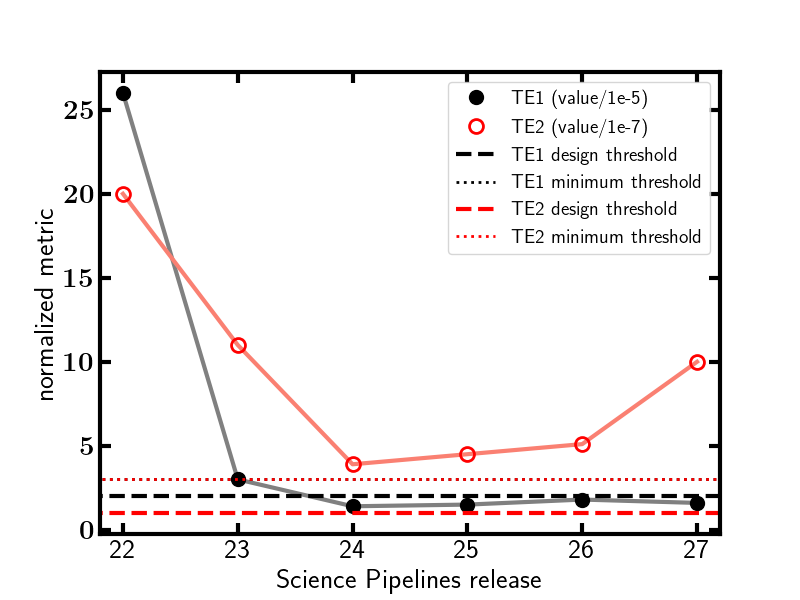
\includegraphics[width=0.6\textwidth, trim=0.0in 0.0in 0.0in 0.0in, clip]{figures/ellip_metrics_v27_with_thresholds.png}
  \caption{Median ellipticity residual correlations at 1-arcminute (TE1; normalized by a factor of $1\times10^{-5}$) and 5-arcminute (TE2; normalized by $1\times10^{-7}$) scales, as measured on $r$-band images, compared over the past few major pipelines releases. Measurements are compared against the SRD requirements (for both the ``design'' and ``minimum'' thresholds; note that the normalized minimum thresholds for TE1 and TE2 are the same, and thus indistinguishable on the figure). The measured values of these metrics show little change between v25 and v26, as expected since the shape measurement and PSF estimation algorithms were unchanged between v25 and v26. }
  \label{fig:ellip_metrics}
\end{figure}

The following metrics are defined following LSR-REQ-0097
\citedsp{LSE-29} and Table 27 of \citeds{LPM-17}. Values in this table represent the mean of the results reported by \texttt{faro} for the three tracts in RC2.

Any entries left blank are those for which we do not have data in the given filter for that dataset.

\begin{longtable}[]{@{}llllll@{}}
\toprule
\begin{minipage}[b]{0.12\columnwidth}\raggedright\strut
Metric\strut
\end{minipage} & \begin{minipage}[b]{0.06\columnwidth}\raggedright\strut
Unit\strut
\end{minipage} & \begin{minipage}[b]{0.14\columnwidth}\raggedright\strut
SRD Requirement -- Design\strut
\end{minipage} & \begin{minipage}[b]{0.12\columnwidth}\raggedright\strut
Release 26 Value (RC2) \strut
\end{minipage} & \begin{minipage}[b]{0.12\columnwidth}\raggedright\strut
Release 27 Value (RC2) \strut
\end{minipage} & \begin{minipage}[b]{0.17\columnwidth}\raggedright\strut
Comments\strut
\end{minipage}\tabularnewline
\midrule
\endhead
\begin{minipage}[t]{0.12\columnwidth}\raggedright\strut
TE1: \emph{u}\strut
\end{minipage} & \begin{minipage}[t]{0.06\columnwidth}\raggedright\strut
---\strut
\end{minipage} & \begin{minipage}[t]{0.14\columnwidth}\raggedright\strut
\(\leq 2\times10^{-5}\)\strut
\end{minipage} & \begin{minipage}[t]{0.12\columnwidth}\raggedright\strut
---\strut
\end{minipage} & \begin{minipage}[t]{0.12\columnwidth}\raggedright\strut
--- \strut
\end{minipage} & \begin{minipage}[t]{0.17\columnwidth}\raggedright\strut
No data\strut
\end{minipage}\tabularnewline
\begin{minipage}[t]{0.12\columnwidth}\raggedright\strut
TE1: \emph{g}\strut
\end{minipage} & \begin{minipage}[t]{0.06\columnwidth}\raggedright\strut
---\strut
\end{minipage} & \begin{minipage}[t]{0.14\columnwidth}\raggedright\strut
\(\leq 2\times10^{-5}\)\strut
\end{minipage} & \begin{minipage}[t]{0.12\columnwidth}\raggedright\strut
\(1.8\times10^{-5}\) \strut
\end{minipage} & \begin{minipage}[t]{0.12\columnwidth}\raggedright\strut
\(1.6\times10^{-5}\) \strut
\end{minipage} & \begin{minipage}[t]{0.17\columnwidth}\raggedright\strut
\strut
\end{minipage}\tabularnewline
\begin{minipage}[t]{0.12\columnwidth}\raggedright\strut
TE1: \emph{r}\strut
\end{minipage} & \begin{minipage}[t]{0.06\columnwidth}\raggedright\strut
---\strut
\end{minipage} & \begin{minipage}[t]{0.14\columnwidth}\raggedright\strut
\(\leq 2\times10^{-5}\)\strut
\end{minipage} & \begin{minipage}[t]{0.12\columnwidth}\raggedright\strut
\(1.8\times10^{-5}\)\strut
\end{minipage} & \begin{minipage}[t]{0.12\columnwidth}\raggedright\strut
\(1.6\times10^{-5}\)\strut
\end{minipage} & \begin{minipage}[t]{0.17\columnwidth}\raggedright\strut
\strut
\end{minipage}\tabularnewline
\begin{minipage}[t]{0.12\columnwidth}\raggedright\strut
TE1: \emph{i}\strut
\end{minipage} & \begin{minipage}[t]{0.06\columnwidth}\raggedright\strut
---\strut
\end{minipage} & \begin{minipage}[t]{0.14\columnwidth}\raggedright\strut
\(\leq 2\times10^{-5}\)\strut
\end{minipage} & \begin{minipage}[t]{0.12\columnwidth}\raggedright\strut
\(1.3\times10^{-5}\)\strut
\end{minipage} & \begin{minipage}[t]{0.12\columnwidth}\raggedright\strut
\(2.1\times10^{-5}\)\strut
\end{minipage} & \begin{minipage}[t]{0.17\columnwidth}\raggedright\strut
\strut
\end{minipage}\tabularnewline
\begin{minipage}[t]{0.12\columnwidth}\raggedright\strut
TE1: \emph{z}\strut
\end{minipage} & \begin{minipage}[t]{0.06\columnwidth}\raggedright\strut
---\strut
\end{minipage} & \begin{minipage}[t]{0.14\columnwidth}\raggedright\strut
\(\leq 2\times10^{-5}\)\strut
\end{minipage} & \begin{minipage}[t]{0.12\columnwidth}\raggedright\strut
\(1.1\times10^{-5}\) \strut
\end{minipage} & \begin{minipage}[t]{0.12\columnwidth}\raggedright\strut
\(1.3\times10^{-5}\)\strut
\end{minipage} & \begin{minipage}[t]{0.17\columnwidth}\raggedright\strut
\strut
\end{minipage}\tabularnewline
\begin{minipage}[t]{0.12\columnwidth}\raggedright\strut
TE1: \emph{y}\strut
\end{minipage} & \begin{minipage}[t]{0.06\columnwidth}\raggedright\strut
---\strut
\end{minipage} & \begin{minipage}[t]{0.14\columnwidth}\raggedright\strut
\(\leq 2\times10^{-5}\)\strut
\end{minipage} & \begin{minipage}[t]{0.12\columnwidth}\raggedright\strut
\(2.5\times10^{-5}\)\strut
\end{minipage} & \begin{minipage}[t]{0.12\columnwidth}\raggedright\strut
\(6.4\times10^{-5}\)\strut
\end{minipage} & \begin{minipage}[t]{0.17\columnwidth}\raggedright\strut
\strut
\end{minipage}\tabularnewline
\begin{minipage}[t]{0.12\columnwidth}\raggedright\strut
TE2: \emph{u}\strut
\end{minipage} & \begin{minipage}[t]{0.06\columnwidth}\raggedright\strut
---\strut
\end{minipage} & \begin{minipage}[t]{0.14\columnwidth}\raggedright\strut
\(\leq 1\times10^{-7}\)\strut
\end{minipage} & \begin{minipage}[t]{0.12\columnwidth}\raggedright\strut
---\strut
\end{minipage} & \begin{minipage}[t]{0.12\columnwidth}\raggedright\strut
---\strut
\end{minipage} & \begin{minipage}[t]{0.17\columnwidth}\raggedright\strut
No data\strut
\end{minipage}\tabularnewline
\begin{minipage}[t]{0.12\columnwidth}\raggedright\strut
TE2: \emph{g}\strut
\end{minipage} & \begin{minipage}[t]{0.06\columnwidth}\raggedright\strut
---\strut
\end{minipage} & \begin{minipage}[t]{0.14\columnwidth}\raggedright\strut
\(\leq 1\times10^{-7}\)\strut
\end{minipage} & \begin{minipage}[t]{0.12\columnwidth}\raggedright\strut
\(6.4\times10^{-7}\)\strut
\end{minipage} & \begin{minipage}[t]{0.12\columnwidth}\raggedright\strut
\(7.0\times10^{-7}\)\strut
\end{minipage} & \begin{minipage}[t]{0.17\columnwidth}\raggedright\strut
\strut
\end{minipage}\tabularnewline
\begin{minipage}[t]{0.12\columnwidth}\raggedright\strut
TE2: \emph{r}\strut
\end{minipage} & \begin{minipage}[t]{0.06\columnwidth}\raggedright\strut
---\strut
\end{minipage} & \begin{minipage}[t]{0.14\columnwidth}\raggedright\strut
\(\leq 1\times10^{-7}\)\strut
\end{minipage} & \begin{minipage}[t]{0.12\columnwidth}\raggedright\strut
\(5.1\times10^{-7}\)\strut
\end{minipage} & \begin{minipage}[t]{0.12\columnwidth}\raggedright\strut
\(1.0\times10^{-6}\)\strut
\end{minipage} & \begin{minipage}[t]{0.17\columnwidth}\raggedright\strut
\strut
\end{minipage}\tabularnewline
\begin{minipage}[t]{0.12\columnwidth}\raggedright\strut
TE2: \emph{i}\strut
\end{minipage} & \begin{minipage}[t]{0.06\columnwidth}\raggedright\strut
---\strut
\end{minipage} & \begin{minipage}[t]{0.14\columnwidth}\raggedright\strut
\(\leq 1\times10^{-7}\)\strut
\end{minipage} & \begin{minipage}[t]{0.12\columnwidth}\raggedright\strut
\(4.7\times10^{-7}\)\strut
\end{minipage} & \begin{minipage}[t]{0.12\columnwidth}\raggedright\strut
\(6.7\times10^{-7}\)\strut
\end{minipage} & \begin{minipage}[t]{0.17\columnwidth}\raggedright\strut
\strut
\end{minipage}\tabularnewline
\begin{minipage}[t]{0.12\columnwidth}\raggedright\strut
TE2: \emph{z}\strut
\end{minipage} & \begin{minipage}[t]{0.06\columnwidth}\raggedright\strut
---\strut
\end{minipage} & \begin{minipage}[t]{0.14\columnwidth}\raggedright\strut
\(\leq 1\times10^{-7}\)\strut
\end{minipage} & \begin{minipage}[t]{0.12\columnwidth}\raggedright\strut
\(3.2\times10^{-7}\)\strut
\end{minipage} & \begin{minipage}[t]{0.12\columnwidth}\raggedright\strut
\(6.1\times10^{-7}\)\strut
\end{minipage} & \begin{minipage}[t]{0.17\columnwidth}\raggedright\strut
\strut
\end{minipage}\tabularnewline
\begin{minipage}[t]{0.12\columnwidth}\raggedright\strut
TE2: \emph{y}\strut
\end{minipage} & \begin{minipage}[t]{0.06\columnwidth}\raggedright\strut
---\strut
\end{minipage} & \begin{minipage}[t]{0.14\columnwidth}\raggedright\strut
\(\leq 1\times10^{-7}\)\strut
\end{minipage} & \begin{minipage}[t]{0.12\columnwidth}\raggedright\strut
\(8.8\times10^{-7}\)\strut
\end{minipage} & \begin{minipage}[t]{0.12\columnwidth}\raggedright\strut
\(1.1\times10^{-6}\)\strut
\end{minipage} & \begin{minipage}[t]{0.17\columnwidth}\raggedright\strut
\strut
\end{minipage}\tabularnewline
\bottomrule
\end{longtable}

\section{Computational Performance}\label{computational-performance}

Computational performance metrics were not measured for this release.

\appendix

% Include all the relevant bib files.
% https://lsst-texmf.lsst.io/lsstdoc.html#bibliographies
\section{References} \label{sec:bib}
\renewcommand{\refname}{} % Suppress default Bibliography section
\bibliography{local,lsst,lsst-dm,refs_ads,refs,books}

% Make sure lsst-texmf/bin/generateAcronyms.py is in your path
\section{Acronyms} \label{sec:acronyms}
\addtocounter{table}{-1}
\begin{longtable}{p{0.145\textwidth}p{0.8\textwidth}}\hline
\textbf{Acronym} & \textbf{Description}  \\\hline

CCD & Charge-Coupled Device \\\hline
DM & Data Management \\\hline
DMSR & DM System Requirements; LSE-61 \\\hline
DMTN & DM Technical Note \\\hline
DMTR & DM Test Report \\\hline
DRP & Data Release Production \\\hline
FAQ & Frequently Asked Question \\\hline
HSC & Hyper Suprime-Cam \\\hline
HSC-SSP & HSC Subaru Strategic Program \\\hline
KPM & Key Performance Metric \\\hline
LPM & LSST Project Management (Document Handle) \\\hline
LSE & LSST Systems Engineering (Document Handle) \\\hline
LSR & LSST System Requirements; LSE-29 \\\hline
LSST & Legacy Survey of Space and Time (formerly Large Synoptic Survey Telescope) \\\hline
PSF & Point Spread Function \\\hline
Pan-STARRS & Panoramic Survey Telescope and Rapid Response System \\\hline
SRD & LSST Science Requirements; LPM-17 \\\hline
\end{longtable}

% If you want glossary uncomment below and comment out the two lines above.
% \printglossaries

\end{document}
